\documentclass[border=0.2cm, 12pt]{standalone}
\usepackage{tikz}
\usepackage{helvet}
\renewcommand{\familydefault}{\sfdefault}
\usepackage{amsmath, amssymb, amsfonts, mathtools}
\usepackage{color}

\usetikzlibrary{shapes,snakes}
\tikzset{>=latex}

\begin{document}
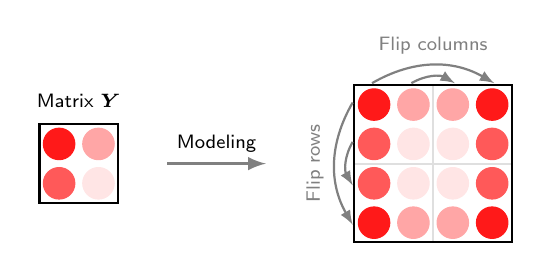
\begin{tikzpicture}

%%% Data matrix X

\node[circle,draw=red!90,fill=red!90,inner sep=0pt,minimum size=0.4cm] (sv1) at (0.25,1.25) {};
\node[circle,draw=red!10,fill=red!10,inner sep=0pt,minimum size=0.4cm] (sv1) at (0.75,0.75) {};
\node[circle,draw=red!65,fill=red!65,inner sep=0pt,minimum size=0.4cm] (sv1) at (0.25,0.75) {};
\node[circle,draw=red!35,fill=red!35,inner sep=0pt,minimum size=0.4cm] (sv1) at (0.75,1.25) {};
\draw [thick] (0,0.5) rectangle (1,1.5);

\node at (0.5,1.8) {\scriptsize\color{black}Matrix $\boldsymbol{Y}$};

\node at (2.25,1.25) {\scriptsize\color{black}Modeling};
\node (G) at (1.5,1) {};\node (H) at (3,1) {};\draw [->,very thick,gray] (G) edge (H);

%%% Big matrix
\newcommand{\temp}{4}

%%% (1,1)-th block
\node[circle,draw=red!90,fill=red!90,inner sep=0pt,minimum size=0.4cm] (sv1) at (0.25+\temp,1.75) {};
\node[circle,draw=red!10,fill=red!10,inner sep=0pt,minimum size=0.4cm] (sv1) at (0.75+\temp,1.25) {};
\node[circle,draw=red!65,fill=red!65,inner sep=0pt,minimum size=0.4cm] (sv1) at (0.25+\temp,1.25) {};
\node[circle,draw=red!35,fill=red!35,inner sep=0pt,minimum size=0.4cm] (sv1) at (0.75+\temp,1.75) {};
\draw [thick,color=gray!25] (0+\temp,1) rectangle (1+\temp,2);

%%% (2,1)-th block
\node[circle,draw=red!65,fill=red!65,inner sep=0pt,minimum size=0.4cm] (sv1) at (0.25+\temp,0.75) {};
\node[circle,draw=red!35,fill=red!35,inner sep=0pt,minimum size=0.4cm] (sv1) at (0.75+\temp,0.25) {};
\node[circle,draw=red!90,fill=red!90,inner sep=0pt,minimum size=0.4cm] (sv1) at (0.25+\temp,0.25) {};
\node[circle,draw=red!10,fill=red!10,inner sep=0pt,minimum size=0.4cm] (sv1) at (0.75+\temp,0.75) {};
\draw [thick,color=gray!25] (0+\temp,0) rectangle (1+\temp,1);

%%% (1,2)-th block
\node[circle,draw=red!35,fill=red!35,inner sep=0pt,minimum size=0.4cm] (sv1) at (1.25+\temp,1.75) {};
\node[circle,draw=red!65,fill=red!65,inner sep=0pt,minimum size=0.4cm] (sv1) at (1.75+\temp,1.25) {};
\node[circle,draw=red!10,fill=red!10,inner sep=0pt,minimum size=0.4cm] (sv1) at (1.25+\temp,1.25) {};
\node[circle,draw=red!90,fill=red!90,inner sep=0pt,minimum size=0.4cm] (sv1) at (1.75+\temp,1.75) {};
\draw [thick,color=gray!25] (1+\temp,1) rectangle (2+\temp,2);

%%% (2,2)-th block
\node[circle,draw=red!10,fill=red!10,inner sep=0pt,minimum size=0.4cm] (sv1) at (1.25+\temp,0.75) {};
\node[circle,draw=red!90,fill=red!90,inner sep=0pt,minimum size=0.4cm] (sv1) at (1.75+\temp,0.25) {};
\node[circle,draw=red!35,fill=red!35,inner sep=0pt,minimum size=0.4cm] (sv1) at (1.25+\temp,0.25) {};
\node[circle,draw=red!65,fill=red!65,inner sep=0pt,minimum size=0.4cm] (sv1) at (1.75+\temp,0.75) {};
\draw [thick,color=gray!25] (1+\temp,0) rectangle (2+\temp,1);

\draw [thick] (0+\temp,0) rectangle (2+\temp,2);

\node (G) at (0.05+\temp,1.4) {};\node (H) at (0.05+\temp,0.6) {};\draw [->, thick,gray] (G) edge[bend right] (H);
\node (G) at (0.05+\temp,1.9) {};\node (H) at (0.05+\temp,0.1) {};\draw [->, thick,gray] (G) edge[bend right] (H);

\draw (-0.5+\temp,1) node[rotate = 90] {\scriptsize{\color{gray}Flip rows}};

\node (G) at (0.6+\temp,1.95) {};\node (H) at (1.4+\temp,1.95) {};\draw [->, thick,gray] (G) edge[bend left] (H);
\node (G) at (0.1+\temp,1.95) {};\node (H) at (1.9+\temp,1.95) {};\draw [->, thick,gray] (G) edge[bend left] (H);
\draw (1+\temp,2.5) node {\scriptsize{\color{gray}Flip columns}};

\end{tikzpicture}
\end{document}